\documentclass[fontsize=12pt,paper=usletter,open=any,
  twoside=no,toc=listof,toc=bibliography,
  captions=nooneline,captions=tableabove,english,DIV=calc,numbers=noenddot,final,parskip=full,
  headinclude=true,footinclude=false,BCOR=0mm,heading=normal]{scrartcl}

\pdfvariable suppressoptionalinfo 512\relax
\interfootnotelinepenalty=10000
\synctex=1

\usepackage[english]{babel}

\author{Valentin Boettcher}
\usepackage{hirostyle}
\usepackage{hiromacros}
\addbibresource{references.bib}

\newcommand{\vc}[1]{\ensuremath{\symbf{#1}}}
\newcommand{\mt}[1]{\ensuremath{\underline{\symbf{#1}}}}

\title{Mode Splitting in Coupled Fibres}
\date{\today}
\graphicspath{{graphics}}
\usetikzlibrary{external}

\begin{document}
\maketitle
\tableofcontents
\begin{figure}[h]
  \centering
  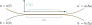
\includegraphics{fibre_coupler}
  \caption{Schematic of the fibre coupler that couples two fibers with
  mode amplitudes \(a\) and \(b\) via an altered transversal
  refractive index \(ε^{*}\) that's only nonzero on a spatial region
  of length \(Δz\). The \(a\) mode is iluminated
  and couples into the \(b\) mode. Here the case for \(n=0\) in
  \cref{eq:16} is shown. The yellow line symbolizes the power of the
  electromagnetic field. }
  \label{fig:schem}
\end{figure}

In the following, we will derive a first-order formula for the mode
splitting of two weakly coupled fiber loops, based on
\cite{Snyder1972}. The usual performance characteristic of a fiber
coupler that is specified the manufacturer is the power splitting.
Consider the situation in \cref{fig:schem}. Outsize of the region
\(Δz\) we have two separate fibers, modelled as cylindrical
wave-guides with a single transversal mode (\(m_{i}= \{a,b\}\)) each
without loss of generality. The electric field in those regions will
take the the form
\begin{equation}
  \label{eq:1}
  \vb{E}(x,y,z;ω) =  m_{i}(z;ω) \vb{e}_{i}(x,y)
\end{equation}
for an arbitrary \(ω\). The vectors
\(\vb{e}_{i}\) are transverse to the fiber axis and describe the
transverse profile of the modes in the two fibers.

Now, the two fiber-cores are brought into close contact over a region
\(Δz\). In that region their transversal permittivity profile will be
perturbed from \(ε \to ε^{*}(z)\) and the solutions to the transverse
Maxwell equations will be altered. The method proposed in
\cite{Snyder1972} is now to expand the solution altered Maxwell
equations in terms of the original modes. To that end, one allows the
\(m_{i}\) in \cref{eq:1} to acquire a spatial dependence.

This leads in this simplified case where only one transverse mode is
considered to the simple equation~\cite{Snyder1972}
\begin{equation}
  \label{eq:2}
  \dv{m_{i}(z)}{z} - \iu \frac{ω}{c} m_{i}(z) = iω ∑_{j} C_{ij}(z) m_{j}(z)
\end{equation}
for sufficiently small coupling \(\epsilon\).
The coupling coefficients \(C_{ij}\) can be calculated from first
principles, but we will assume
\begin{equation}
  \label{eq:3}
  C_{12}(z)=C_{21}(z)=\epsilon θ(z)θ(Δz-z).
\end{equation}

For the boundary condition \(m_{1}(0)=a(0)=a_{0}\neq0\) and
\(m_{2}=b(0)=0\) we find for the mode amplitudes at the output ports
\begin{equation}
  \label{eq:5}
  \begin{aligned}
    a'=a(Δz) & = \cos(ω Δz \epsilon) & b'=b(Δz) = \sin(ω Δz \epsilon).
  \end{aligned}
\end{equation}
Thus, the power simply gets transferred between the fibers in an
oscillatory fashion. The resulting power splitting is then
\begin{equation}
  \label{eq:4}
  s = \abs{\frac{b(Δz)}{a(Δz)}}^{2} = \tan[2](ω Δz \epsilon).
\end{equation}
It is clear that the same power splitting can be achieved with
different \(Δz\), while keeping \(\epsilon\) fixed. The concrete
implementation is down to the manufacturer. A further ambiguity is
that a splitting ratio reported, for example, as \(25:75\) could mean
\(s=75/25\) or \(s=25/75\) in terms of the definition in
\cref{eq:4}. All in all we can deduce
\begin{equation}
  \label{eq:16}
  ωΔz \epsilon = \tan[-1](\sqrt{s}) + n π,
\end{equation}
where \(n\in\ZZ\).

We now wish to derive how the resonator frequencies of two fiber loops
change when they are coupled by the fiber coupler described above. To
that end, we assume that the loops have the lengths
\begin{equation}
  \label{eq:6}
  L=L_{1}= N L_{2}
\end{equation}
where \(N\) is an integer.
In the uncoupled case, the mode amplitudes now fulfill periodic
boundary conditions
\begin{equation}
  \label{eq:8}
  m_{i}(0) = m_{i}(L_{i}).
\end{equation}
We can thus expand the longitudinal mode profiles \(m_{i}\) in a
Fourier series
\begin{equation}
  \label{eq:9}
  \begin{aligned}[b]
    a(z) & = ∑_{n} a_{n} \eu^{\iu k_{n}z} & k^{(i)}_{n} & = \frac{2π}{L_{1}}n \\
    b(z) & = ∑_{n} b_{n} \eu^{\iu q_{n}z} & q^{(i)}_{n} & = \frac{2π}{L_{2}}n
  \end{aligned}%
  \qq{with} n\in\ZZ
\end{equation}
Inserting this into the coupled mode equations of \cref{eq:2},
we obtain
\begin{equation}
  \label{eq:10}
  \begin{aligned}
    \mt{M}\pmqty{\vc{a}                \\\vc{b}} \equiv \pmqty{\mt{k}-\frac{ω}{c} & -\frac{ω}{L_{1}} \mt{C} \\ -\frac{ω}{L_{2}} \mt{{C}}^{\intercal} &
    \mt{q} -\frac{ω}{c}} \pmqty{\vc{a} \\\vc{b}}
  \end{aligned}=\vc{0},
\end{equation}
where \(\mt{k}\;(\mt{q})\) are diagonal matrices with the
\(k_{n}\; (q_{n})\) on the diagonal. The bold \(\vb{a}\) and
\(\vb{b}\) are the vectors with the Fourier components \(a_{n}\) and
\(b_{n}\) as their coefficients. The coupling matrices are defined as
follows from \cref{eq:3}
\begin{equation}
  \label{eq:11}
  \mt{C}_{m,n} = ∫_{0}^{Δz}C_{12}(z)\eu^{-\iu \pqty{k_{m}-q_{n}}z}\dd{z}.
\end{equation}

By finding the solutions to \(\det[\mt{M}]=0\), we can identify the
mode frequencies of the resonators. To simplify the calculation we
will assume that the wavelengths of all relevant modes are much
shorter than \(Δz\) (i.e. \(\abs{q_{m}-k_{n}} \gg Δz^{-1}\) for all
relevant \(n,\,m\)) and that thus only modes with \(k_{m}=q_{n}\)
couple. As \(k_{N n} = q_{n}\) for \(n\in \ZZ\), we have
\begin{equation}
  \label{eq:13}
  \mt{C}_{m,n} =
  \begin{cases}
    \epsilon Δz & \text{if}\; m = N \times n \\
    0           & \text{otherwise}.
  \end{cases}
\end{equation}
We then have
\begin{equation}
  \label{eq:14}
  \det[\mt{M}] = f(\mt{k}) \det[\pqty{\mt{q} -\frac{ω}{c}}^{2} -
  \frac{\pqty{ω\epsilon Δz}^{2}}{L_{1}L_{2}} \id].
\end{equation}
The roots of the determinant corresponding to the hybridized modes are
\begin{equation}
  \label{eq:15}
  \begin{aligned}[t]
    ω_{\pm} & = \frac{1}{2α} \pqty{\frac{q_{n}}{c} \pm \sqrt{\pqty{\frac{q_{n}}{c}}^{2} - 4α q_{n}^{2}}} \\
            & = c q_{n} \pqty{1 \pm \frac{cΔz \epsilon}{\sqrt{L_{1}L_{2}}}} +
    \mathcal{O}\pqty{\epsilon^{2}}                                                                       \\
            & \equiv ω_{n} \pm δ
  \end{aligned}
\end{equation}
with \(α=c^{-2}-\epsilon Δz/(L_{1} L_{2})\).
The thus find that the bare frequencies of the small loop are split
with
\begin{equation}
  \label{eq:17}
  δ = ω_{n} \frac{cΔz \epsilon}{\sqrt{L_{1}L_{2}}} = ω_{n}Δz \epsilon\frac{\sqrt{Ω_{1}Ω_{2}}}{2π}
\end{equation}
with the free spectral ranges of the fiber loops
\begin{equation}
  \label{eq:18}
  Ω_{i} = \frac{2π c}{L_{i}}.
\end{equation}
With the help of \cref{eq:16} and remembering that
\begin{equation}
  \label{eq:20}
  Ω_{2} = N Ω_{1} = Ω = \frac{2πc}{L}
\end{equation}
we can express the mode splitting \(δ\)
as
\begin{equation}
  \label{eq:19}
  δ = \frac{\sqrt{N}Ω}{2π}\pqty{\tan[-1](\sqrt{s}) + n π},
\end{equation}
where \(s\) is the splitting ratio, \(Ω\) is the free spectral range
of the big loop and \(n\in \ZZ\).

Often, \(n=0\) corresponding to the case where the power never fully
oscillates into the second fiber. Also, when in doubt, it may be
useful to try \(s^{-1}\) as it's not always clear which output port of
the fiber coupler corresponds to which fiber.

As an example \(s=75/25\) and \(n=0\) gives \(\frac{δ}{Ω} = 0.167\)
which is reasonably close to the value determined \(δ/Ω = 0.171\)
in~\cite{Pellerin2023}\footnote{The \(δ\) given in the paper
  corresponds to \(2δ\) in this note's notation.}.

\printbibliography
\printindex
\end{document}


%%% Local Variables:
%%% mode: latex/mps
%%% TeX-master: t
%%% TeX-output-dir: "output"
%%% TeX-engine: luatex
%%% jinx-languages: "en_CA"
%%% End:
